%results


                \begin{figure}[!ht]
		\begin{center}
		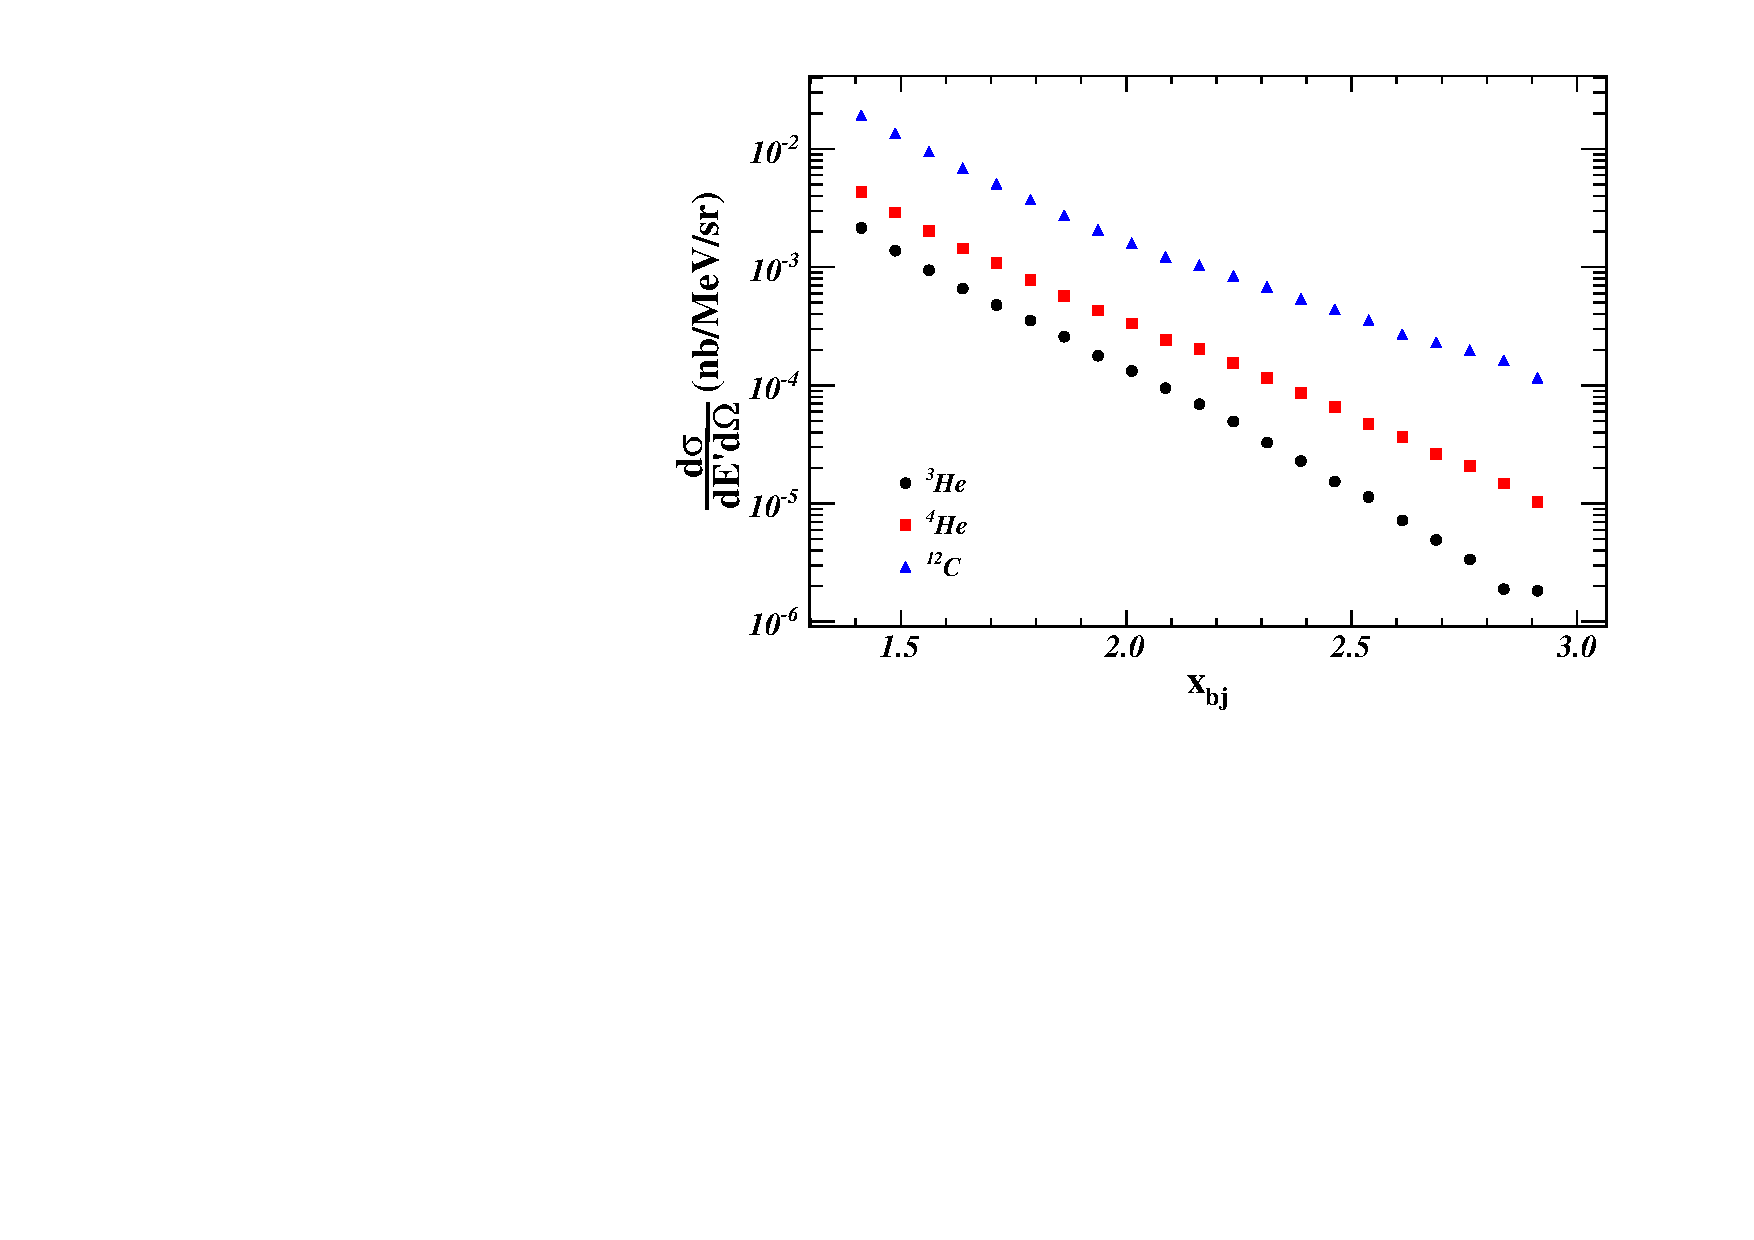
\includegraphics[height=9.0cm,angle=270]{./figures/XS_Comp_25_May27}
		\end{center}
		\vspace*{-5mm}
		\caption{(Color online) Cross sections of $^{3}$He, $^{4}$He and $^{12}$C at $25^{\circ}$. The uncertainties include statistical and
		systematic uncertainties. An additional normalization uncertainty of XX\% is not shown.}
		\label{xs}
		\end{figure}

The absolute cross sections for scattering from $^{3}$He, $^{4}$He and $^{12}$C at a scattering angle of $25^{\circ}$ are shown in Fig.~\ref{xs}.


                \begin{figure}[!ht]
		\begin{center}
		  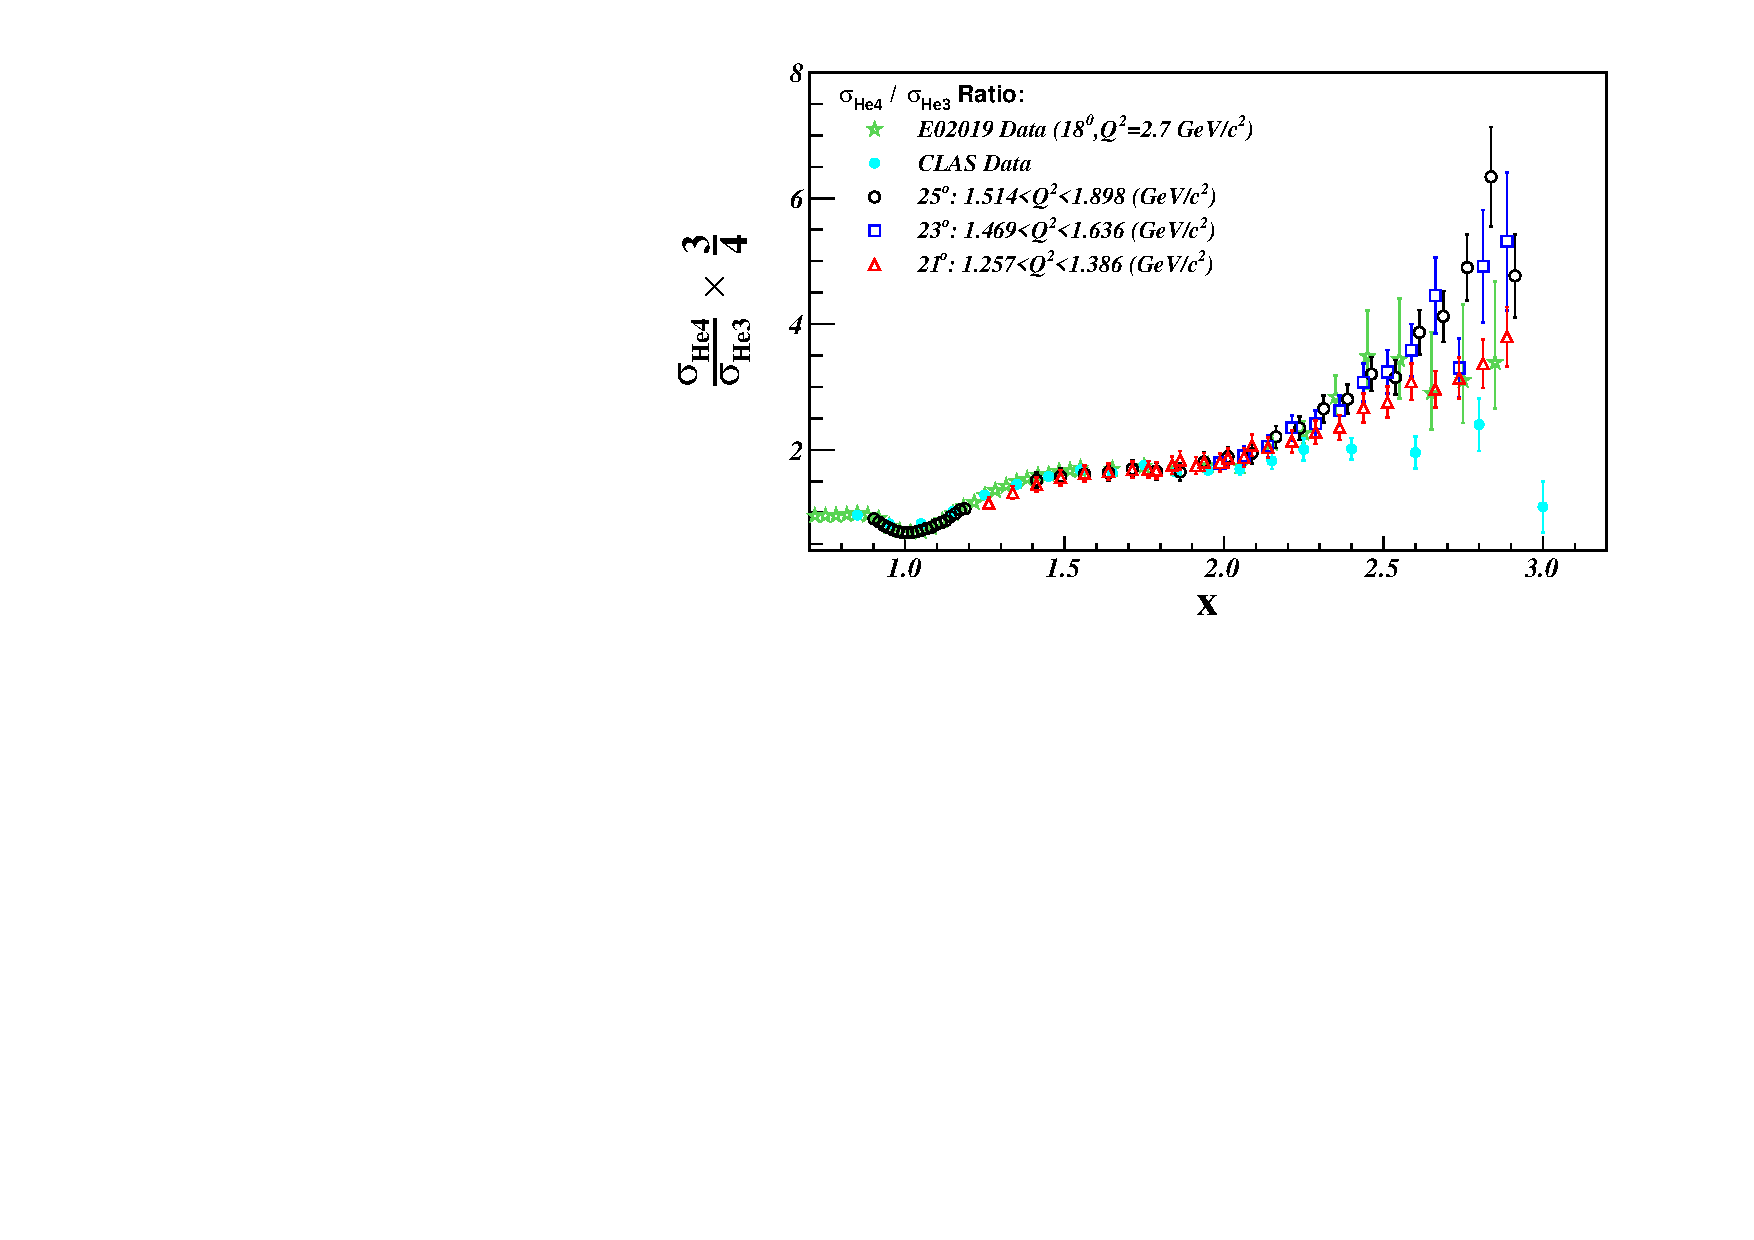
\includegraphics[height=9.5cm,angle=270]{./figures/He4_He3_XS_Ratio_June30_L}
                  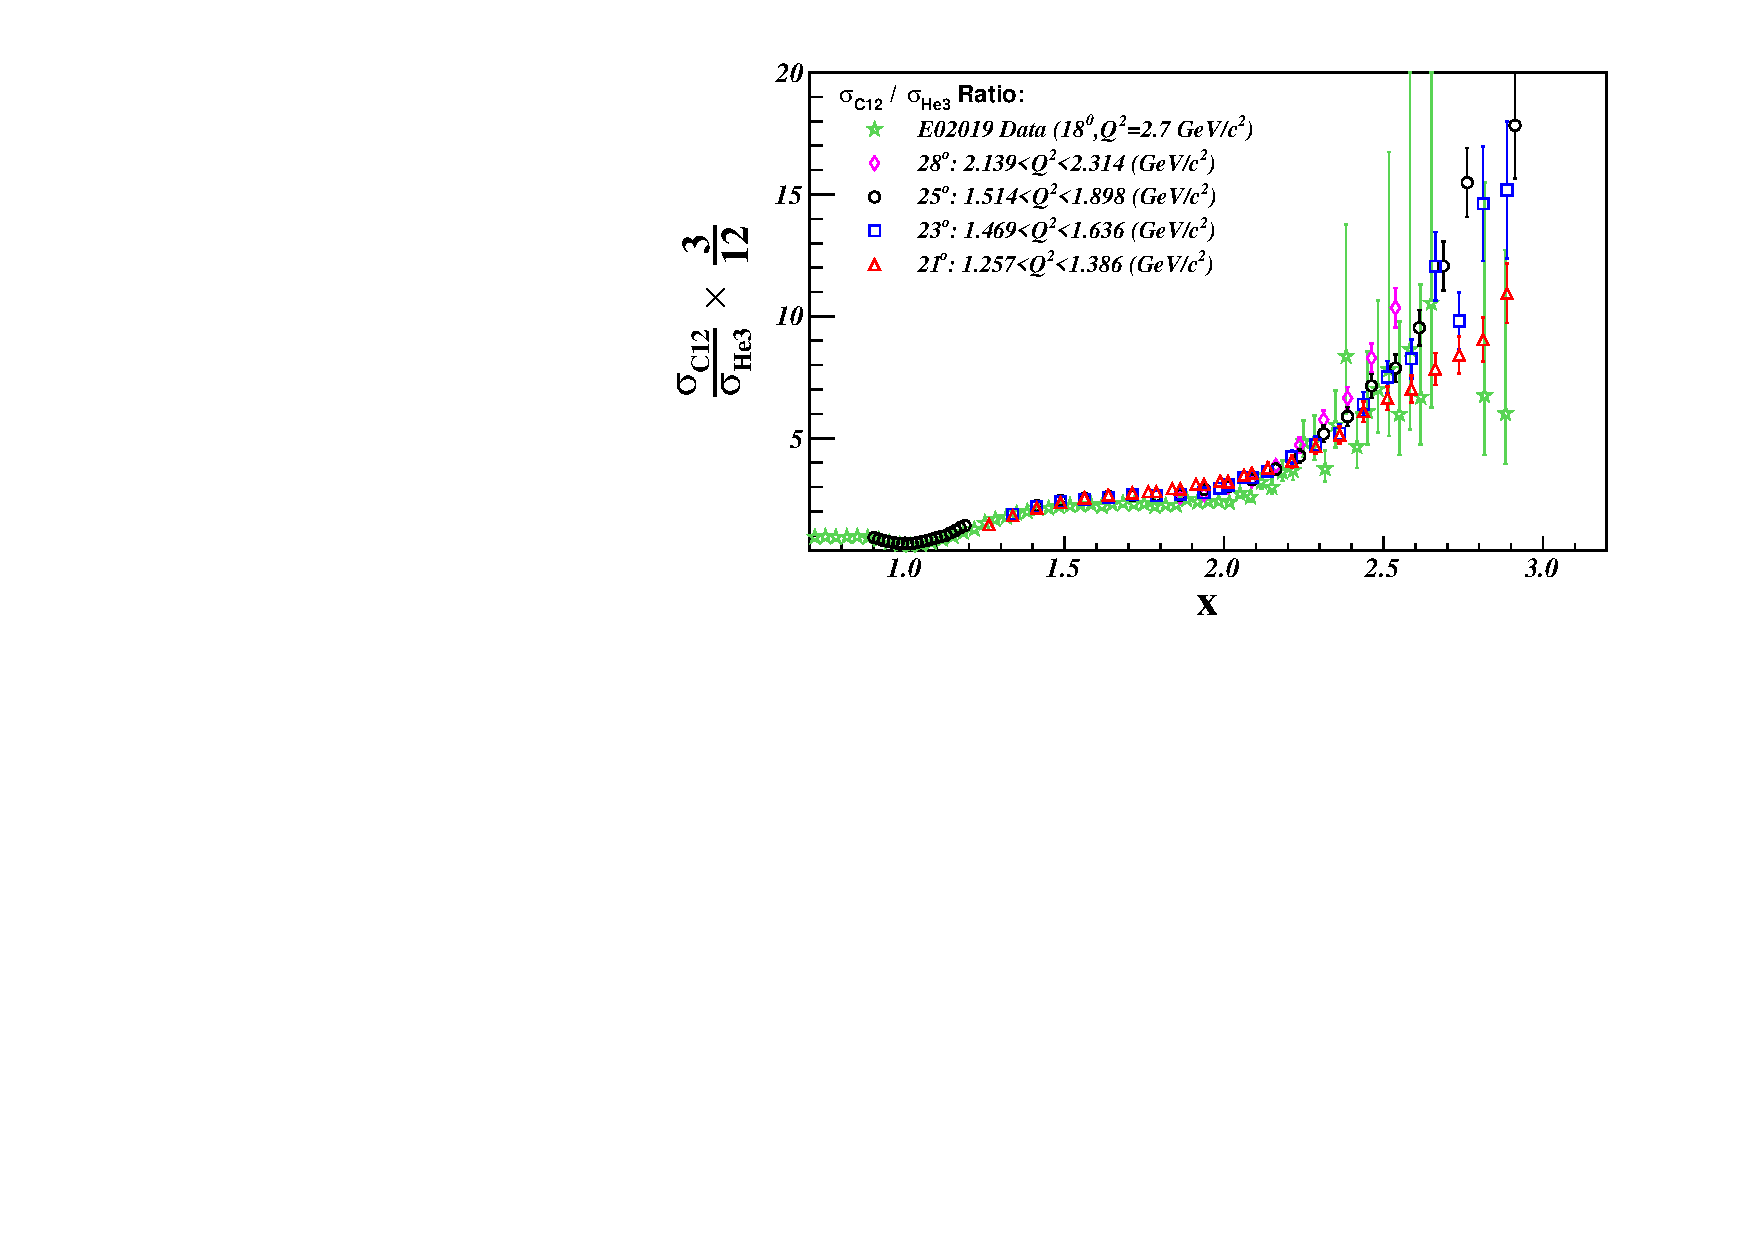
\includegraphics[height=9.5cm,angle=270]{./figures/C12_He3_XS_Ratio_June30_L}
%                  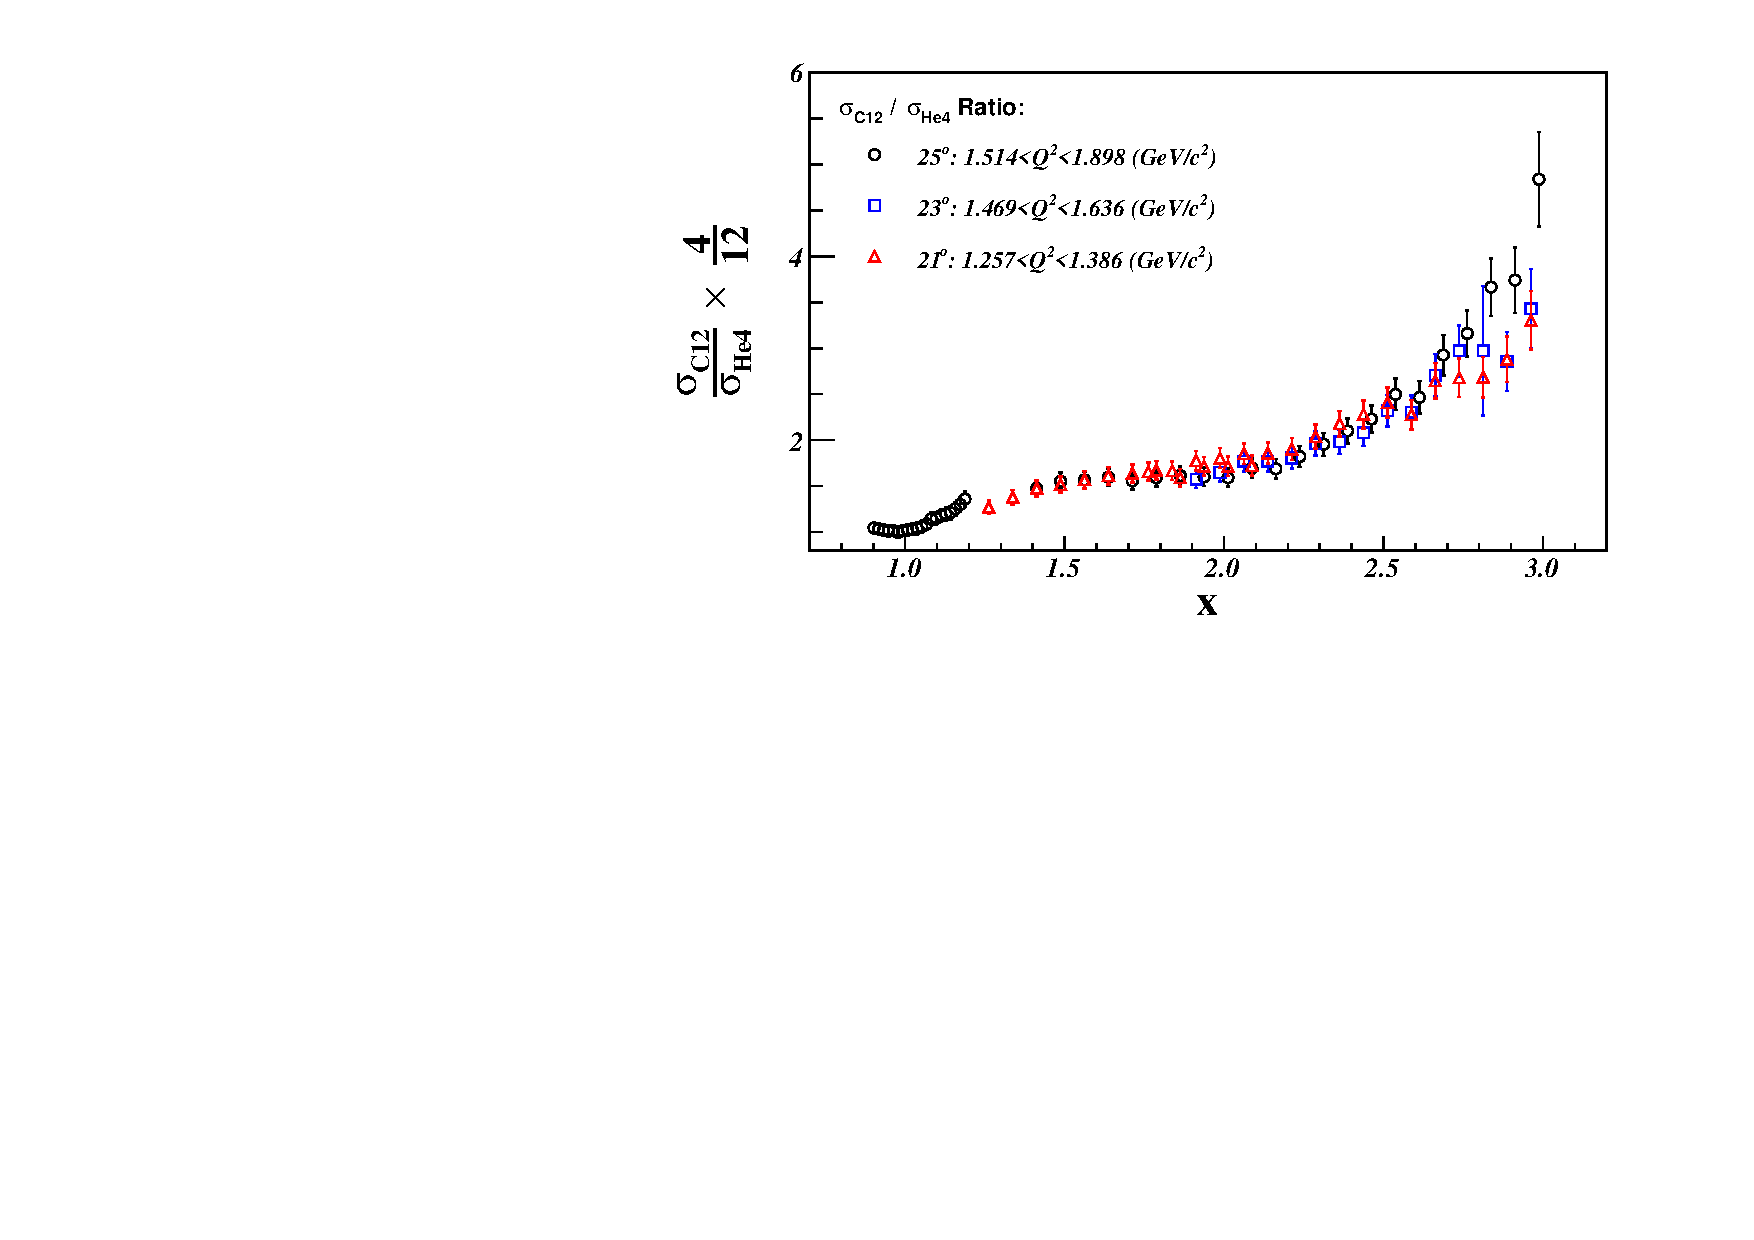
\includegraphics[height=9.0cm,angle=270]{./figures/C12_He4_XS_Ratio_June30_L}
		\end{center}
		\vspace*{-5mm}
		\caption{(Color online) The $^4$He/$^3$He (top) and $^{12}$C/$^3$He (bottom) cross section ratios for this
		  measurement, along with results from CLAS~\cite{PhysRevLett.96.082501} and Hall C (E02-019)~\cite{fomin2012} measurements.
                  Uncertainties include statistical and systematic uncertainties. A normalization uncertainty of XX\% (top) and YY\% (bottom)
		  is not included. \textit{JRA: It will be good to make these large, so making the y-axis labels less 'tall' will help, e.g.
		  something like $(\sigma_{4He}/4)/(\sigma_{3He}/3)$. Do we want to include our cross section model to show $Q^2$ dependence?}}
		\label{ratios}
		\end{figure}

Fig.~\ref{ratios} presents the ratio of the $^4$He and $^{12}$C cross sections to $^3$He as a function of $x$. In the 2N-SRC region, our data
are in good agreement with the data from CLAS~\cite{PhysRevLett.96.082501} and E02-019~\cite{fomin2012}, revealing a plateau between $x \approx
1.5$ and $x = 2$. At $x>2$, our ratios are significantly larger than the CLAS ratios, and in generally good agreement with the E02-019 ratios.
The disagreement between the CLAS ratios and both our results and the E02-019 data suggest a problem with the extracted ratios from
Ref.~\cite{PhysRevLett.96.082501} above $x=2$. A recent comment~\cite{Higinbotham:2014xna} suggested that the 3N-SRC plateau showed in the CLAS
data could be a result of inappropriate binning and bin-centering correction.

We observe a small but systematic $Q^2$ dependence in our data, and do not see indications of a well defined 3N-SRC plateau. Instead our ratios
show a slow rise above $x=2$, with a more rapid increase as $x \to 3$, suggesting that the simple model of 3N-SRC dominance is not valid in this
region. While this behavior does not match the prediction of the native 3N-SRC model, namely A/$^3$He ratios independent of $x$ and $Q^2$ for $x
\gtorder 2.5$, this does not provide a clear demonstration that 3N-SRCs are unimportant in this region.

For 2N-SRCs, the prediction of scaling is relatively straightforward and robust. One can predict \textit{a priori} where the plateau should be
observed since for any given $Q^2$, a value of $x$ can be selected that corresponds to a minimum nucleon momentum that is above the Fermi
momentum, thus suppressing the mean-field contributions. As one approaches $x=2$, the plateau will disappear as the deuteron cross section falls
to zero and so the A/$^2$H ratios must rise sharply to infinity. For both the data and our simple cross section model, based on a calculated
deuteron momentum distribution, this does not occur until $x \approx 1.9$, yielding a clear plateau for $1.5 < x < 1.9$.

In attempting to isolate 3N-SRC contributions, the situation is less straightforward. Both 2N and 3N SRCs yield contributions to the 
high-momentum tail. The fact that we do not see significant deviations from the 2N-SRC picture for $1.5<x<2$ suggests that the 3N-SRC
contributions are generally much smaller. Unlike the case for 2N-SRCs, where $k>k_F$ suppresses single particle strength, there is
not a clear way to define a threshold in $x$ that will sufficiently suppress
2N contributions.  Approaching the kinematic limit at $x \approx 3$, the $^3$He cross section falls to zero and the ratio must go to
infinity. However, while this occurs in a vary narrow $x$ window for the A/$^2$H ratios, the rise occurs over a larger range in $x$
in this case.

Thus, it is not clear that there will be a significant window in $x$ where one would expect to see a plateau, especially at the relatively modest
$Q^2$ values measured here. In the present experiment, we observe a small but noticeable $Q^2$ dependence, in particular for $x \gtorder 2.5$. This
is also observed in our simple $y$-scaling cross section model, and does not occur in the $^{12}$C/$^3$He ratio, indicating that it is the $x$
dependence of the falloff of the $^3$He cross section as $x \to 3$ that is varying strongly with $Q^2$. Larger $Q^2$ values may be required to
observe a $Q^2$-independent behavior of the ratios with $x$, which may allow us to isolate 3N-SRC contributions.



\textit{Figure with A/2H ratios up to $x=2$, table with $a_2$ results for $A=3$, 4, 12, 48?}


%JRA Notes:
%0) Can we look at A/D ratios vs. Q^2 for our cross section model? Impact of x-->2 in 2H? Where does A/D rise up for x-->2?
%1) x-->3 has may have larger missing energy (plus, smaller energy step from x=1 to 2 to 3, so may fall to zero over wider range.
%2) $Q^2$ dependence of $x \to 3$ ratios in general agreement with what we observe in our cross section model. Suggests that the cross
%section falloff as we approach the kinematic threshold is large
